
\section{Introduction}
%
Glimmer-CISM\footnote{{\it Glimmer} was originally an acronym, reflecting the project's origin within the GENIE climate model. The meaning of the Glimmer acronym is no longer important but reflects the current codes origins within the Glimmer project. CISM stands for Community Ice Sheet Model, and reflects the project's evolution towards a fully supported, coupled component of the \href{http://www2.cesm.ucar.edu/}{Community Earth System Model}, or CESM.} is a numerical model - a collection of software libraries, utilities and drivers  - used to simulate ice sheet evolution. Glimmer-CISM is modular in design and coded almost entirely in standards-complient Fortran 95 \textbf{SP:should this be F90?}. It has two different ``dynamical cores", which solve the equations for the conservation of mass, energy, and momentum. As with previous versions of Glimmer, the serial, shallow-ice representation of ice dynamics is still supported, through the GLIDE dynamical core. New with Glimmer-CISM is the GLISSADE dynamical core, which supports higher-order ice dynamics, scalable parallelism, and includes software links for coupling to robust, third-party solver libraries. 
%
\section{Overview}
%
Glimmer-CISM consists of several components:
%
\begin{itemize}
\item {\bf GLIDE:} {\bf G}eneral {\bf L}and {\bf I}ce {\bf D}ynamic {\bf E}lements: the dynamical core for the model based on shallow-ice dynamics. This component is responsible for solving the governing conservation equations and determining ice velocities, internal ice temperature distribution, and ice geometry evolution (see Chapter \ref{ch:glide}). In addition, GLIDE components determine isostatic adjustment and meltwater production. GLIDE needs some representation of the climate to run, provided by a {\it driver} program. The user may write their own driver code, or may use one of the four supplied drivers (see section \ref{subsec:climdrive}). \textbf{SP: some of this is not accurate or may need to be rewritten}
\item {\bf GLISSADE:} {\bf acronymn for this?}: the dynamical core for the higher-order model based on the 1st-order accurate Stokes approximation. As with GLIDE, this component is responsible for solving the governing conservation equations. Unlike GLIDE, the GLISSADE dynamical core is fully parallel to take advantage of modern, multi-processor, high-performance architectures  (see Chapter \ref{ch:glissade}).
\item {\bf GLINT:} {\bf GL}IMMER {\bf Int}erface. Originally developed for the GENIE %\footnote{Grid-ENabled Integrated Earth-system model} 
Earth Systems Model, GLINT allows the core ice model to be coupled to a variety of global climate models, or indeed any source of time-varying climate data on a lat-long grid. An example driver is provided to illustrate the use of GLINT, which uses temperature and precipitation data to drive a positive degree day (PDD) mass-balance model.
\item {\bf shared, high-hevel code:} I'm thinking of stuff like derived types (glide types), config file parser (glide setup), i/o, build system files, etc. Would rather avoid giving it a cute name (like Glum, which I think is supposed to encompass this kind of stuff, but sounds stupid)
\item {\bf SIMPLE:} Simple climate drivers that implement the experiments of the first phase of the EISMINT project, with idealised geometry. \textbf{SP: suggest we call this something else? Simple doesn't really make much sense any more. Should this whole item simply be renames "test cases"?}
%% SP: commented out the remainder, since we aren't supporting these anymore (and GLUM is included above, w/o the silly name)
%\item {\bf EIS:} {\bf E}dinburgh {\bf I}ce {\bf S}heet climate driver based on a parameterisation of the equilibrium line altitude, sea-level surface temperatures and eustatic sea-level change. \textbf{SP: Not used/supported anymore - remove?}
%\item {\bf EISMINT3:} An implementation of a later part of the EISMINT project, concerning the modelling of the Greenland ice sheet. 
%\item {\bf GLUM:} {\bf G}Limmer {\bf U}seful {\bf M}odules, various utility procedures used by the other components. 
%\item Visualisation programs using GMT\footnote{Generic Mapping Tools}. 
\end{itemize}
%
%\begin{figure}[htbp]
%  \centering
%  \includegraphics[width=0.6\textwidth]{\dir/figs/Glimmer.eps}
%  \caption{Relationship between the various Glimmer components.}
%  \label{ug.fig.Glimmer}
%\end{figure}
*** This is all old below here and needs to be redone ***

The relationship between the Glimmer components is illustrated in Figure \ref{ug.fig.Glimmer}. 
%
\subsection{Climate Drivers}
\label{subsec:climdrive}
The core ice sheet model, GLIDE, is connected to the climate via the surface mass balance and temperature fields and (optionally) a scalar value for eustatic sea level. These drivers can be derived from simple assumptions, e.g. uniform mass balance or EISMINT tests, or from climate model output, e.g. GENIE or a regional climate model. These components, and how they relate to each other, are outlined in Figure \ref{ug.glide}.
%
%\begin{figure}[htbp]
% \begin{center}
%   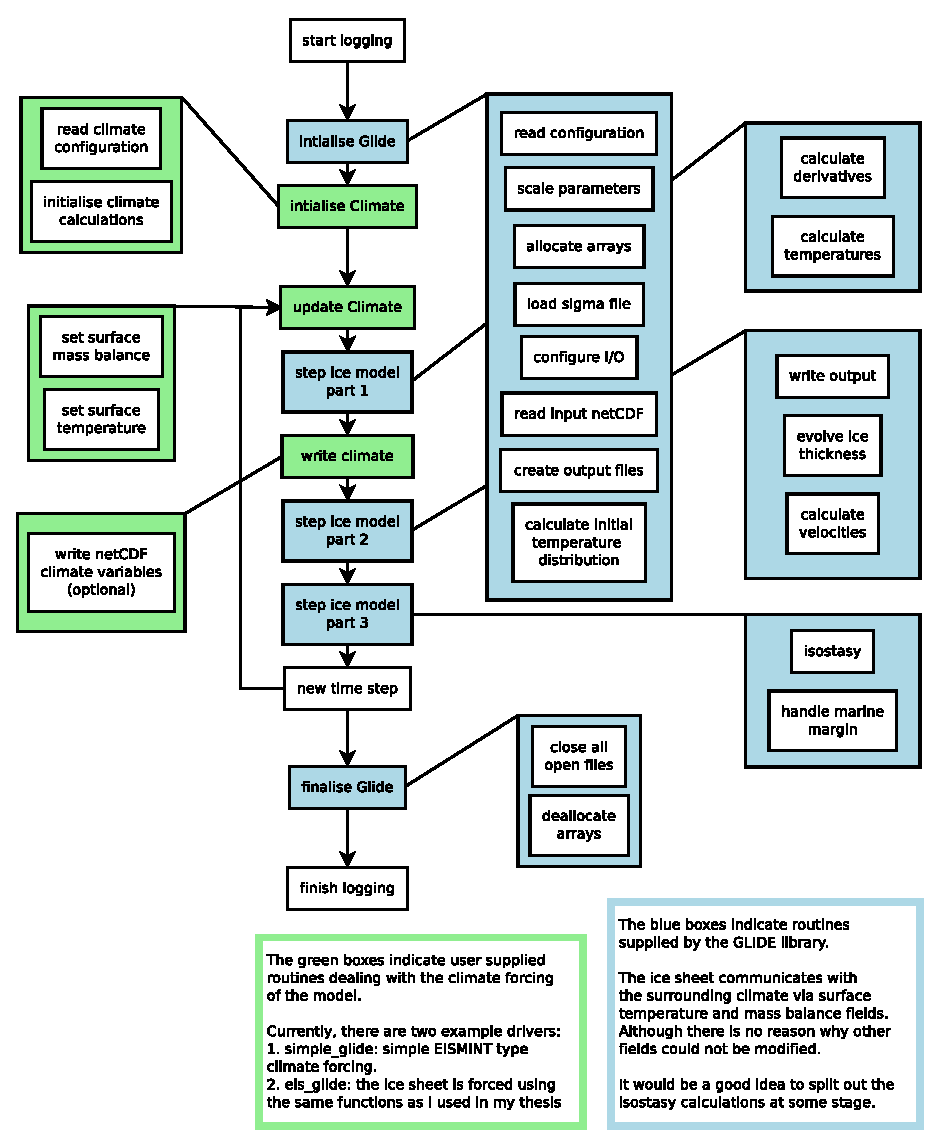
\includegraphics[width=0.9\textwidth]{\dir/figs/glide.eps}
% \end{center}
% \caption{Outline of the GLIDE and Climate components.}
%\label{ug.glide}
%\end{figure}
%
\subsection{Configuration, I/O and Visualisation}
In general terms, each component is configured using a configuration file similar to Windows \texttt{.ini} files. At run-time, model configuration is printed to a log file. 

2D and 3D data is read/written to/from netCDF files using the CF (Climate-Forecast) metadata convention\footnote{\texttt{http://www.cgd.ucar.edu/cms/eaton/cf-metadata/}}. NetCDF is a scientific data format for storing multidimensional data in a platform- and language-independent binary format. The CF conventions specify the metadata used to describe the file contents.

Many programs can process and visualise netCDF data, e.g. OpenDX, Matlab, IDL, etc. Additionally, the Glimmer code bundle contains GMT scripts written in Python to visualise the output.
